% TU Delft Beamer template
% Author: Maarten Abbink
% Delft University of Technology
% March 2014
% Version 2.0
% Based on original version 1.0 of Carl Schneider
\documentclass{beamer}
\usepackage[utf8]{inputenc}
\usepackage[T1]{fontenc}
\usepackage[brazil]{babel}
\usepackage{calc}
\usepackage{pbox}
\usepackage[absolute,overlay]{textpos}

% colors for links
\definecolor{links}{HTML}{2A1B81}
\hypersetup{colorlinks,linkcolor=blue,urlcolor=links}

\mode<presentation>{\usetheme{tud}}

\title[SDN]{SDN e as inovações em rede}
%\subtitle
\institute{DCC - UFMG}
\author{Gustavo Pantuza}
\date{01 de Novembro}


% define a symbol which can be removed if you don't need it
\newcommand{\field}[1]{\mathbb{#1}}
\newcommand{\Zset}{\field{Z}}

\begin{document}

{
% remove the next line if you don't want a background image
\usebackgroundtemplate{
\includegraphics[width=\paperwidth,height=\paperheight]{images/networking.jpg}}
\setbeamertemplate{footline}{\usebeamertemplate*{minimal footline}}
\frame{\titlepage}
}


%
% Introduction
%
\section{Introdução}


%
% Community emvolvment
%
\begin{frame}\frametitle{Apresentação}

	\begin{figure}[h]
        \centering
        
\includegraphics[scale=0.5]{images/community.png}
    \end{figure}
\end{frame}


%
% Motivation
%
\begin{frame}\frametitle{Motivação}
   
    \begin{itemize}
        \setlength{\itemsep}{1cm}
        \item A Internet demanda que a infraestrutura evolua em paralelo com 
            as aplicações e serviços
        \item Algoritmos em grafos são base para diversas aplicações em rede
        \item Computação feita em diferentes nós da rede repetidamente
        \item Logicamente centralizado, o plano de controle permite 
            minimizar a quantidade de computações
    \end{itemize}
\end{frame}


%
% Problem
%
\begin{frame}\frametitle{Problema}
    \begin{itemize}
        \setlength{\itemsep}{1cm}
        \item Uma visão topológica global é um dos principais aspectos do 
              paradigma das Redes definidas por software.
        \item Grafos representam de maneira natural e precisa a topologia 
            de uma rede.
        \item Grafos deveriam ser um recurso básico, uma premissa em 
            controladores SDN
    \end{itemize} 
\end{frame}


%
% Scientific contributions
%
\begin{frame}\frametitle{Contribuições científicas}
    \begin{itemize}
        \setlength{\itemsep}{1cm}
        \item Uma abstração da rede na forma de um grafo dinamicamente 
            atualizado.
        \item Avaliações do controlador, da rede e do protocolo OpenFlow
        \item Avaliação de grafos como primitiva em SDN
    \end{itemize}
\end{frame}

\section{SDN}



%
% SDN
%
\begin{frame}\frametitle{SDN}

    \begin{itemize}
    \item SDN é apenas um modelo
    \vspace*{0.5cm}
    \item Um \emph{design} para construção e administração de redes
    \vspace*{0.5cm}
    \item A separação dos planos de controle e de dados torna o 
          funcionamento da rede mais flexível
    \end{itemize}
\end{frame}

%
% SDN
%
\begin{frame}\frametitle{Características}

    \begin{itemize}
    \item Torna a rede programável
    \vspace*{0.1cm}
    \item Flexibilidade na administração da rede
    \vspace*{0.1cm}
    \item Controle logicamente centralizado
    \vspace*{0.1cm}
    \item Configurável via programação
    \vspace*{0.1cm}
    \item Padronização aberta 
    \end{itemize}
\end{frame}


%
% Openflow
%
\begin{frame}\frametitle{Openflow}

    \begin{itemize}
    \item Se SDN é só um modelo, como implementá-lo?
    \end{itemize}
    	\begin{figure}[h]
        \centering
        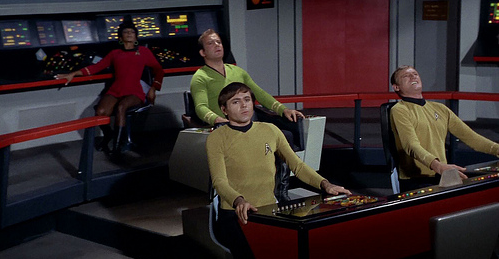
\includegraphics[scale=0.5]{images/control-room.png}
    \end{figure}
\end{frame}



%
% Openflow
%
\begin{frame}\frametitle{Openflow}

    \begin{itemize}
    \item Openflow é um protocolo que possibilita experimentos e aplicações
          em SDN
    \end{itemize}
    	\begin{figure}[h]
        \centering
        
\includegraphics[scale=0.3]{images/openflow.png}
    \end{figure}
\end{frame}


%
% Openflow
%
\begin{frame}\frametitle{Openflow}

    \begin{itemize}
    \item \href{http://archive.openflow.org/documents/openflow-wp-latest.pdf}{Artigo} publicado em 2008 
    \item Permitiu que pesquisadores pudessem criar experimentos com novos
          protocolos em redes convencionais 
    \end{itemize}

\end{frame}




%
% Openflow
%
\begin{frame}\frametitle{Porque é tão importante?}

    \begin{itemize}
    \item A arquitetura da Internet tem deficiências
    \item Inovações em rede custam caro
    \item A arquitetura continua acoplada à infraestrutura
    \item O Openflow define um padrão que qualquer fabricante de     
          \emph{hardware} de rede pode implementar
    \end{itemize}

\end{frame}

\section{architecture}


%
% Archtecture
%
\begin{frame}\frametitle{Arquitetura Openflow}

    \begin{itemize}
    \item Temos dois papeis principais:
        \begin{itemize}
        \item Controlador
        \item Switch Openflow
        \end{itemize}
    \item Algo te lembra plano de dados e controle desacoplados?
    \end{itemize}
    
	\begin{figure}[h]
        \centering
        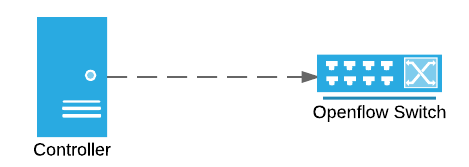
\includegraphics[scale=0.6]{images/controller-to-openflow.png}
    \end{figure}
\end{frame}



%
% Switch Archtecture
%
\begin{frame}\frametitle{Arquitetura do Switch Openflow}

    \begin{itemize}
    \item Internamente um Switch openflow é assim:
    \end{itemize}
    
	\begin{figure}[h]
        \centering
        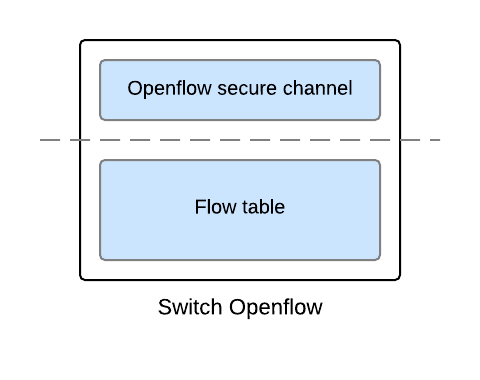
\includegraphics[scale=0.5]{images/openflow-switch-architecture.png}
    \end{figure}
\end{frame}

%
% Switch Archtecture
%
\begin{frame}\frametitle{Arquitetura Openflow}

    \begin{itemize}
    \item \textbf{Openflow secure channel}: É a conexão segura entre o
          controlador e o switch openflow
    \vspace*{0.5cm}
    \item \textbf{Flow table}: É a tabela onde são identificados os fluxos
    \vspace*{0.5cm}
    \item Para cada fluxo tem-se uma ação (action) a ser tomada
    \end{itemize}
\end{frame}

%
% Switch Archtecture
%
\begin{frame}\frametitle{Arquitetura Openflow}

    \begin{itemize}
    \item Um fluxo é identificado pelos seguintes campos do cabeçalho 
          Openflow:
    \end{itemize}
	\begin{figure}[h]\hspace*{-1.2cm}
        \centering
        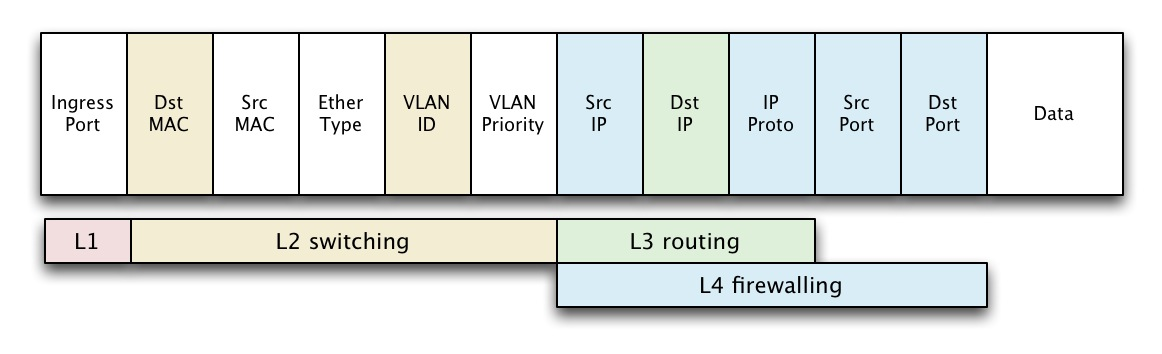
\includegraphics[scale=0.32]{images/openflow-header.jpg}
    \end{figure}
    
\end{frame}


%
% Actions
%
\begin{frame}\frametitle{Actions}

	\begin{figure}[h]
        \centering
        
\includegraphics[scale=0.5]{images/action.png}
    \end{figure}
    
\end{frame}


%
% Actions
%
\begin{frame}\frametitle{Tipos de Actions}

    \begin{itemize}
    \item Forwarding
    \item Drop
    \item Set
    \item strip
    \item Copy-in
    \item Copy-out
    \item Push
    \item Pop
    \item Dec
    \end{itemize}

\end{frame}


%
% Flow table 
%
\begin{frame}\frametitle{Tabela de Fluxos}

\begin{center}
    \begin{tabular}{ | l | l | l | l |}
    \hline
    \textbf{Header} & \textbf{Counters} & \textbf{Actions} & \textbf{Priority} \\ \hline
    in\_port=5 & 55635 bytes & \pbox{20cm}{Forward \\ port=8} & 100 \\ \hline
    \pbox{20cm}{ip=192.168.1.42 \\ port=80} & 4032 bytes & \pbox{30cm}{Set \\ rewrite \\ ip=192.168.1.100} & 500 \\ \hline
    ipproto=UDP & 100 bytes & Drop & 700 \\ \hline
    \end{tabular}
\end{center}

\end{frame}

%
% Controller
%
\begin{frame}\frametitle{Controlador}

    \begin{itemize}
    \item É um software que se conecta de maneira segura ao switch openflow
          com o objetivo de manipular sua tabela de fluxos
    \item Esse software pode ser distribuído
    \item Ele representa uma entidade lógica e centralizada
    \item É possível ter visão e controle de estado global da rede
    \item Permite que outros serviços e programas façam requisições e troca
          de mensagem com o plano de controle da rede
    \item Pode calcular estatísticas da rede
    
    \end{itemize}

\end{frame}


%
% Controller
%
\begin{frame}\frametitle{Controlador}

    \begin{itemize}
    \item Cabe ao programador lidar com os problemas típicos em 
          desenvolvimento de software:
          \begin{itemize}
          \item Tolerância a falha
          \item Persistência
          \item Eficiência
          \item design de implementação
          \item debugging
          \item Testes
          \end{itemize}
    \end{itemize}
\end{frame}

%
% Controller
%
\begin{frame}\frametitle{Controlador}

    \begin{itemize}
    \item Controladores Openflow:
          \begin{itemize}
          \item Biblioteca \href{http://opennetworkingfoundation.github.io/libfluid/index.html}{Libfluid}
                para criação de aplicações/controladores em SDN
          \item \href{http://www.noxrepo.org/nox/about-nox/}{Nox Controller}
          \item \href{https://openflow.stanford.edu/display/Beacon/Home}{Beacon}
          \item \href{http://www.noxrepo.org/pox/about-pox/}{Pox Controller}
          \item \href{http://osrg.github.io/ryu/}{Ryu}
          \end{itemize}
    \end{itemize}
\end{frame}


%
% Simple topology
%
\begin{frame}\frametitle{Arquitetura Openflow}

    \begin{itemize}
    \item Uma topologia simples:
    \end{itemize}
    
	\begin{figure}[h]
        \centering
        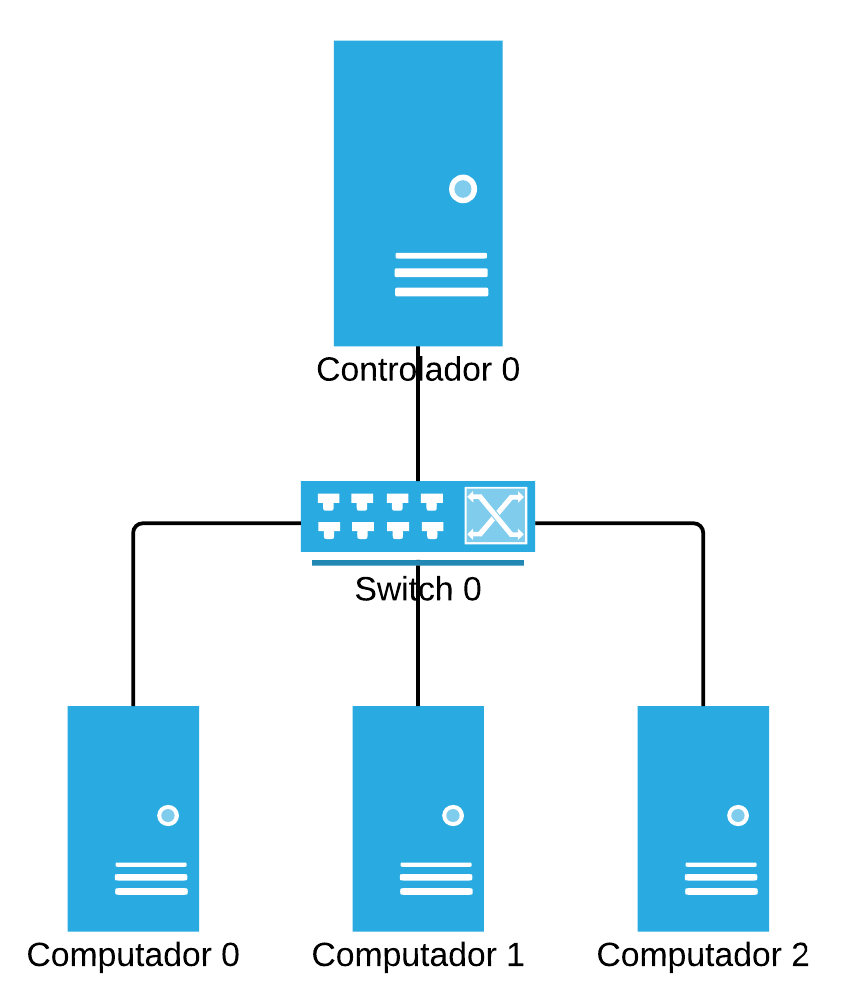
\includegraphics[scale=0.3]{images/simple-topology.png}
    \end{figure}
\end{frame}


%
% N openflow 
%
\begin{frame}\frametitle{Arquitetura Openflow}

    \begin{itemize}
    \item Um controlador para vários \emph{Switches}
    \end{itemize}
    
	\begin{figure}[h]
        \centering
        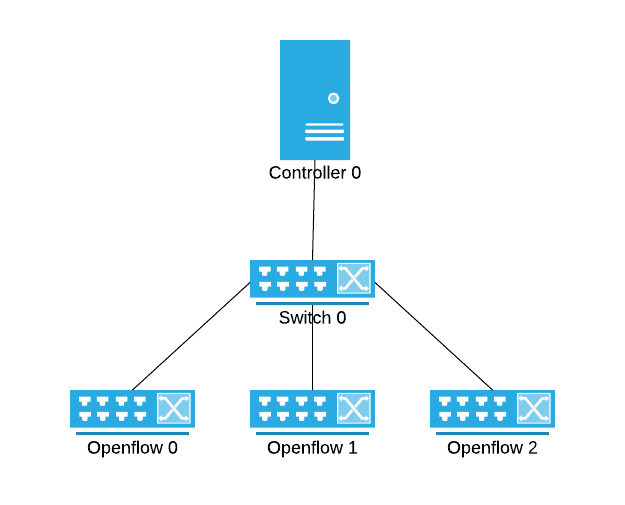
\includegraphics[scale=0.4]{images/n-openflow-switches.png}
    \end{figure}
\end{frame}


%
% SDN inter domain
%
\begin{frame}\frametitle{Arquitetura Openflow}

    \begin{itemize}
    \item Comunicação entre domínios de rede
    \end{itemize}
    
   
	\begin{figure}[h]\hspace*{-1cm}
        \centering
        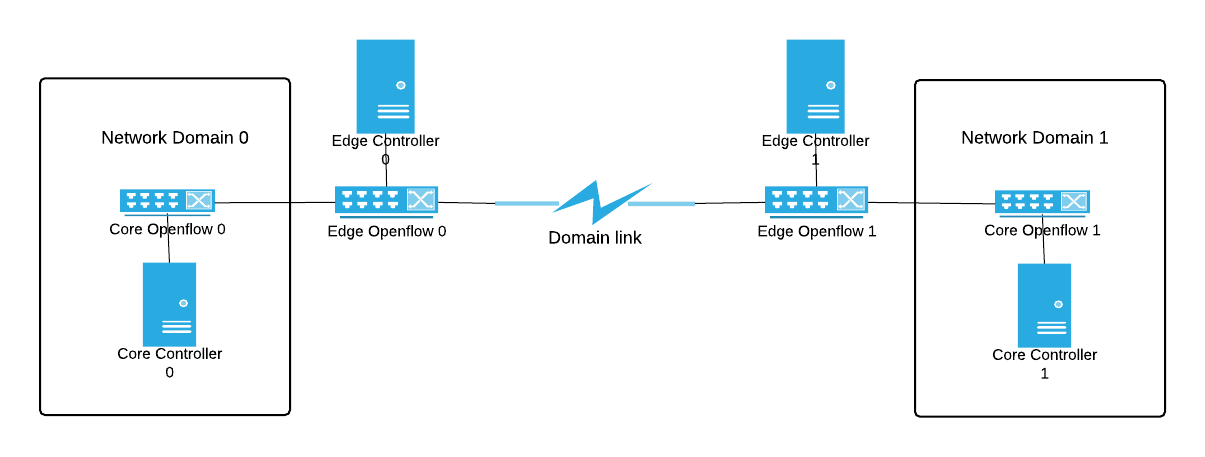
\includegraphics[scale=0.3]{images/edge-core-sdn.png}
    \end{figure}
\end{frame}



%
% Distributed openflow controller
%
\begin{frame}\frametitle{Arquitetura Openflow}

    \begin{itemize}
    \item Controlador distribuído
    \end{itemize}
    
	\begin{figure}[h]
        \centering
        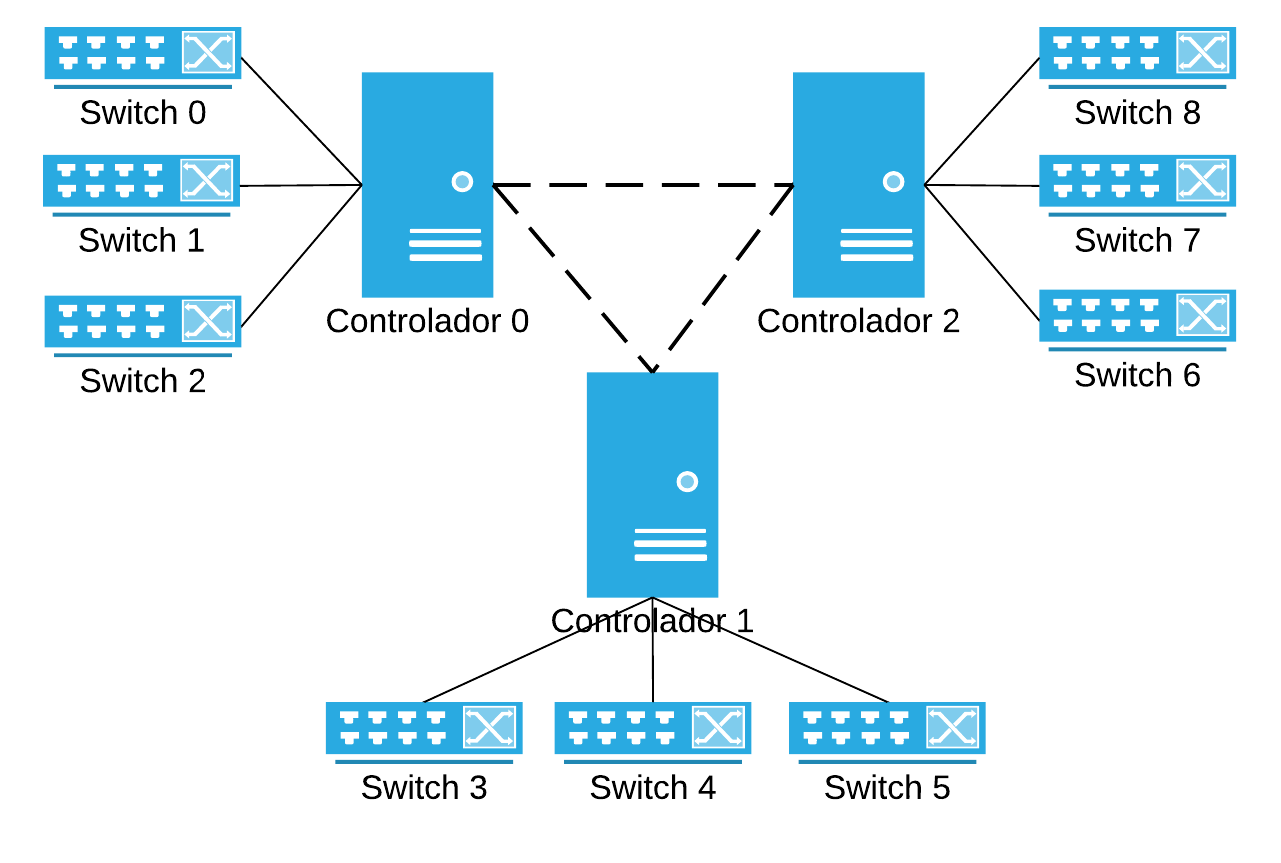
\includegraphics[scale=0.4]{images/distributed_sdn_controller.png}
    \end{figure}
\end{frame}
\section{Market}

%
% Market
%
\begin{frame}\frametitle{Mercado}

	\begin{figure}[h]\hspace*{1cm}
        \centering
        
\includegraphics[scale=1.0]{images/onf.png}
    \end{figure}
\end{frame}


%
% ONF members
%
\begin{frame}\frametitle{Mercado}

    \begin{itemize}
    \item Quem participa da ONF
    \end{itemize}
    	\begin{figure}[h]\hspace*{-0.3cm}
        \centering
        
\includegraphics[scale=0.35]{images/onf-board.png}
    \end{figure}
\end{frame}


%
% ONF members
%
\begin{frame}\frametitle{Mercado}

    	\begin{figure}[h]
        \centering
        
\includegraphics[scale=0.2]{images/notbad.png}
    \end{figure}
\end{frame}


%
% Openflow vendors
%
\begin{frame}\frametitle{Fabricantes}

	\begin{figure}[h]
        \centering
        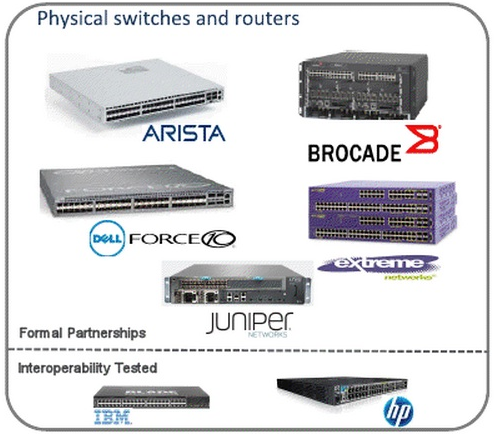
\includegraphics[scale=0.4]{images/of-vendors.png}
    \end{figure}
\end{frame}



%
% Virtual Openflow vendors
%
\begin{frame}\frametitle{Fabricantes}

	\begin{figure}[h]
        \centering
        
\includegraphics[scale=0.4]{images/of-virtual-vendors.png}
    \end{figure}
\end{frame}


%
% ONF members
%
\begin{frame}\frametitle{Mercado}

    	\begin{figure}[h]
        \centering
        
\includegraphics[scale=0.6]{images/trap.jpg}
    \end{figure}
\end{frame}


%
% Experiment world wide
%
\begin{frame}\frametitle{Case}
    \begin{itemize}
    \item Google Openflow network
    \end{itemize}
	\begin{figure}[h]\hspace*{-0.5cm}
        \centering
        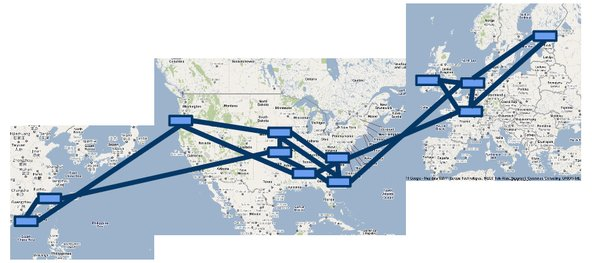
\includegraphics[scale=0.5]{images/google-sdn.jpg}
    \end{figure}
\end{frame}

\chapter{Trabalhos futuros}
\label{chap:future-work}

Como uma proposta futura, criar visualizador em tempo real do grafo que 
interaja com o administrador da rede e mostre, de uma maneira simples, 
toda a operação da rede.

Assim como o controlador POX, o módulo proposto, ao ter seu processo terminado,
não persiste as informações de estado da rede.
Todo o grafo computado é perdido.
Em função disso, um banco de dados em grafos, distribuído, poderia ser 
utilizado para persistir o grafo, e as informações do estado da rede, de 
maneira confiável e tolerante a falhas. 

Algoritmos genéricos em grafos poderiam ser implementados como uma biblioteca
para o módulo.
Assim, estabelecida uma periodicidade, esses algoritmos poderiam ser computados
no grafo e seus resultados publicados como extensão da API.

\section{Questions}

\begin{frame}
  {Dúvidas?}

\begin{figure}[h]\vspace*{-1cm}
    \centering
    
\includegraphics[scale=0.2,width=\linewidth]{images/questions}
\end{figure}

Contatos:
    \begin{columns}[T] % align columns
        \begin{column}{.57\textwidth}
            \begin{itemize}
                \item email: \href{mailto:gustavopantuza@gmail.com}{gustavopantuza@gmail.com}
                \item github: \href{http://github.com/pantuza}{pantuza}
            \end{itemize}
        \end{column}%
        \hfill%
        \begin{column}{.43\textwidth}
            \begin{itemize}
                \item twitter: \href{http://twitter.com/gpantuza}{@gpantuza}
                \item site: \href{http://pantuza.com}{http://pantuza.com}
            \end{itemize}
        \end{column}%
    \end{columns}
\end{frame}



\end{document}
